\section{Sequenzdiagramme}

\begin{figure}[h!]
\begin{center}
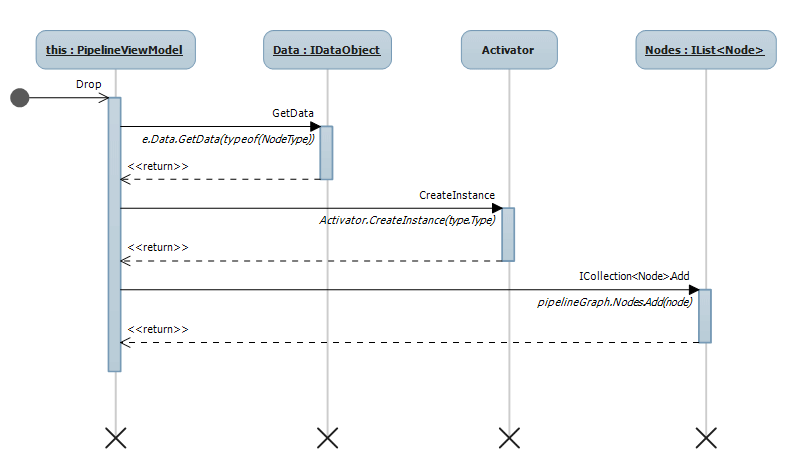
\includegraphics[height=0.7\textheight]{Diagrams/drop.png}
\end{center}
\caption{Hinzufügen eines Knotens}
\end{figure}

\begin{figure}[h!]
\begin{center}
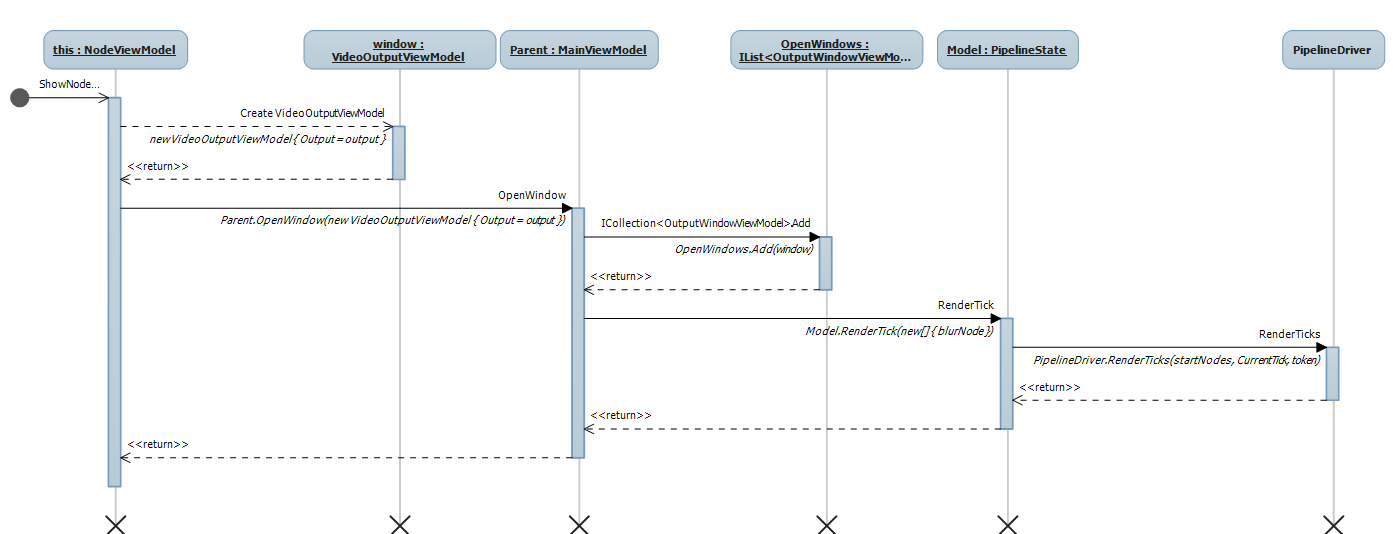
\includegraphics[height=0.9\textheight]{Diagrams/shownodeoutput.png}
\end{center}
\caption{Hinzufügen eines Ausgabefensters}
\end{figure}

\begin{figure}[h!]
\begin{center}
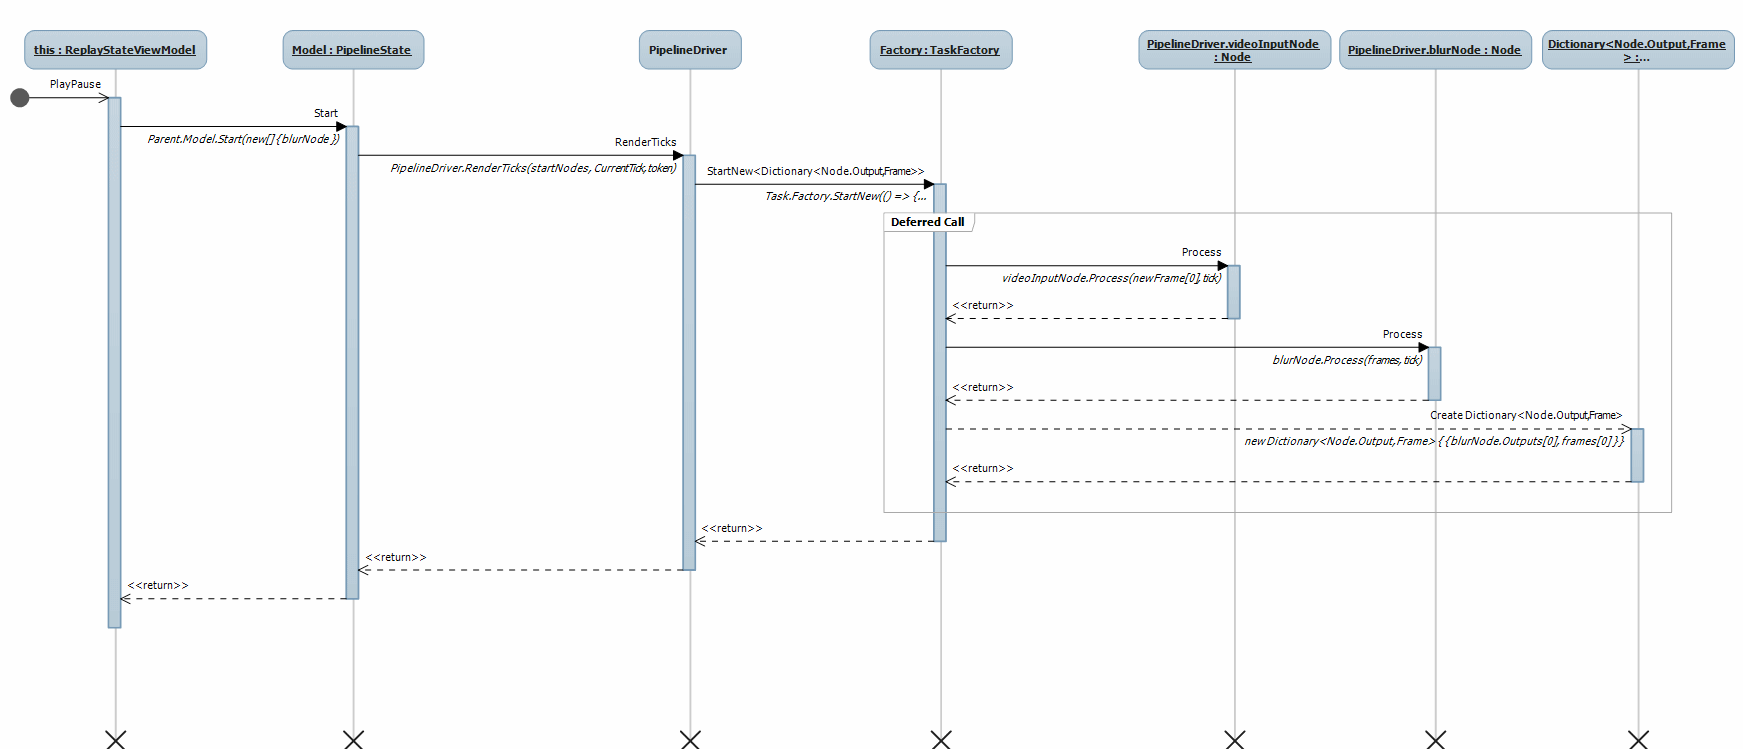
\includegraphics[height=0.9\textheight]{Diagrams/play.png}
\end{center}
\caption{Abspielen der Pipeline}
\end{figure}